\chapter{Introduction}\label{ch:intro}

In large-scale \ac{wifi} environments such as office buildings, shopping malls, and airports, where multiple \acp{ap} are required, people often move around indoors with their mobile devices.
To maintain a stable connection to the \ac{wifi}, the station must remain in the range of an \ac{ap} or may roam to another with the same \ac{ssid}.
However, the current roaming process, as defined in the 802.11k/r\cite{802.11k}\cite{802.11r} \ac{wifi} standard, does not consider human movement factors such as acceleration and trajectory.
For example, consider that a user's station moves away from \ac{ap}1 towards \ac{ap}2 and further towards \ac{ap}3, as seen in \Cref{fig:roaming}.
Then, there is no initiation of a roam from \ac{ap}1 to \ac{ap}3, but instead the station will first roam from \ac{ap}1 to \ac{ap}2 and then to \ac{ap}3, which increases the number of roamings leading to interruptions in, e.g, video confereces \cite{handoff_performance_issues}.

\begin{figure}[h]
    \centering
    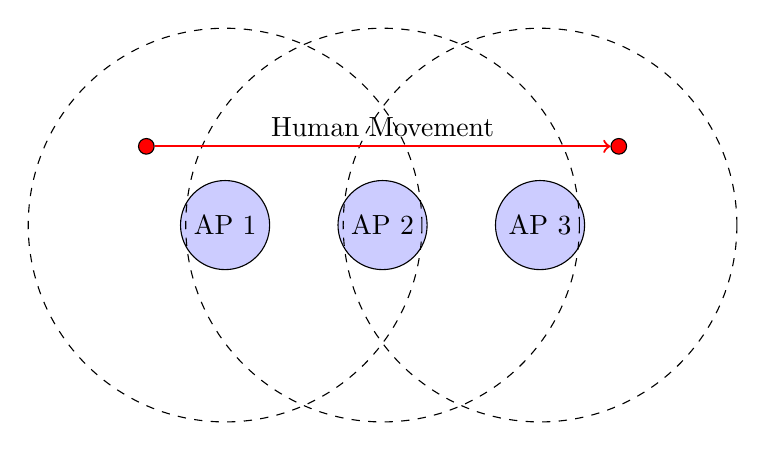
\begin{tikzpicture}
% Access Points
\node[draw, circle, fill=blue!20, minimum size=1cm] (ap1) at (0,0) {AP 1};
\node[draw, circle, fill=blue!20, minimum size=1cm] (ap2) at (2,0) {AP 2};
\node[draw, circle, fill=blue!20, minimum size=1cm] (ap3) at (4,0) {AP 3};

% Ranges
\draw[dashed] (ap1) circle (2.5cm);
\draw[dashed] (ap2) circle (2.5cm);
\draw[dashed] (ap3) circle (2.5cm);

% Person's movement
\node[draw, circle, fill=red, inner sep=2pt] (start) at (-1,1) {};
\node[draw, circle, fill=red, inner sep=2pt] (end) at (5,1) {};
\draw[->, thick, red] (start) -- (end) node[midway, above, black] {Human Movement};
\end{tikzpicture}
    \caption{Roaming process of a user's station from \ac{ap}1 to \ac{ap}3 bypassing also \ac{ap}2.}
    \label{fig:roaming}
\end{figure}

Real-time applications such as video conferencing are susceptible to these frequent roamings, which may result in dropped connections and unsatisfied users.
Reducing the number of roams will reduce the probability of connection losses.
Instead, it would be ideal if the movement from \ac{ap}1 to \ac{ap}3 were detected by the station beforehand and a roam from \ac{ap}1 to \ac{ap}3 was initiated.

Therefore, this thesis explores if a time series \ac{ml} model can predict the following \ac{ap} a station may connect to next.
Because of the many \acp{ap} in large-scale \ac{wifi} environments, I interpret this prediction as a multi-class classification problem where each \ac{bssid} will be a class.
Typical applications for multi-class classification are image recognition of, e.g., animals or handwriting recognition with a limited number of classes \cite{multi-class-classification}.
This thesis has nearly 4800 \acp{bssid}, making the prediction task much more challenging.
Hence, the model predicts a set of three \acp{ap}, defined as \threeAP in the following, that the station may connect to next, which must include the most likely AP to be claimed as a correct prediction.
This prediction will be compared to a heuristic approach, which will choose the following \ac{ap} based on the latest measured \ac{rssi} value.
If the \ac{rssi} is the highest, it is considered the next one to connect to.

A time-series \ac{ml} model requires time series as input.
There are two possible data sources: generate new or utilize existing data. 
Creating a large-scale environment with many \acp{ap} and users is not feasible for this thesis, as this process is time-consuming and needs a lot of planning and evaluation beforehand.
Thus, this thesis will use an existing dataset with sensor data such as acceleration, waypoint, and \ac{wifi} data from large-scale environments.
The only dataset I found meeting these requirements is from a 2021 competition by Microsoft Research \cite{IndoorLocationNavigation}, located on kaggle\footnote{Kaggle, a website containing competitions and datasets for machine learning: \url{https://www.kaggle.com}}.

The prediction will be difficult due to the large number of classes and because multi-class classification, such as image recognition, deals with a limited number of classes.
The more possible classes to be predicted, the more likely a prediction may be wrong.
The relaxation to a \threeAP will make the prediction task easier.
Still, it will be challenging to outperform the heuristic approach, as it is simple because it relies on the last measured \ac{rssi} value, which may not change that much in a short time. 
I expect the \ac{ml} model accuracy to be better than the heuristic approach because we can utilize the user's trajectory, which the heuristic approach cannot.

The rest of this thesis is structured as follows:
In \Cref{ch:background}, I will give an overview of the terms of \ac{ml} concepts and models used in this thesis.
\Cref{ch:related-work} will discuss related work and compares it to this thesis.
The data will be analyzed in \Cref{ch:data-ana} to determine what parts of the data I will use for the \ac{ml} model.
After that, I will discuss the suitability of some pre-selected time series \ac{ml} models for the task in \Cref{ch:discuss-ml}. 
Because of findings in \Cref{ch:data-ana}, this thesis needs to preprocess the prepared data further and will implement the \ac{lstm} model for one site and floor of the competition in \Cref{ch:implementation}.
In \Cref{ch:evaluation}, I will evaluate the model's performance and conclude if this prediction could be useful in the future in \Cref{ch:conclusion}.
